%!TEX root = ../report.tex
\documentclass[../report.tex]{subfiles}

\begin{document}
    \section{Methodology}
    \label{sec:methodology}

    % Describe all conceptual details about your approach in this section.
    % Add any necessary subsections to improve the presentation.

    % Feel free to rename this section to better reflect the concrete topic you are discussing.
    \subsection{Simulation Framework}
    A set of simulation frameworks was investigated to select the best simulation that is available for the project. Gazebo was selected as the simulation based on its compatibility with ROS2 
    and the availability of the plugins that are already made available due to the familiarity of the platform. The SJTU drone system was selected as the drone model for the simulation as it was 
    lightweight and also easy to work with. A new radiation sensor plugin and radiation source plugin were developed to simulate the radiation source and the sensor. This plugin can be easily 
    integrated into the simulation and can be used to simulate the radiation source and the sensor. 
        
    To accurately represent realistic radiation behavior, the radiation source is modeled as a point gamma radiation source that emits radiation uniformly in all directions. The radiation sensor 
    receives and publishes data in the form of photon count rates; however, this count rate is subject to attenuation caused by trees and the air surrounding the sensor. 

    The attenuation from trees is implemented through ray tracing, which helps to determine if the sensor has a clear line of sight to the radiation source. If trees obstruct the line of sight, 
    the radiation is attenuated based on the type of tree and a specific attenuation factor. The positions of the trees are generated dynamically according to the map size while ensuring a 
    maintained specific distance between each tree.
        
    % \subsection{Measurement Model}

    % with measurement model:

    % % mt = Σ(i,j∈Ω) [b(i,j)/((x-xi)^2 + (y-yj)^2 + h^2)] + N(0, 0.5mt)
    % \begin{equation}
    %     m_t = \sum_{i,j \in \Omega} \left[ \frac{b(i,j)}{(x - x_i)^2 + (y - y_j)^2 + h^2} \right] + N(0, 0.5m_t)
    % \end{equation}

    \subsection{Evaluation Framework}

    A new interface for handling the simulation and experiment metrics was developed. The interface is designed with PyQt5, a Python library for creating graphical user interfaces. 
    Two interfaces have been developed that allow one to either handle all the parameters in the workspace or visualize any number of algorithms running within the workspace.
        
    \subsubsection{Parameter Editor}
    The parameter editor application serves multiple purposes beyond the current project. It was developed to provide a unified interface that consolidates all configuration files in YAML format. 
    To ensure compatibility with ROS2 packages, the interface can load the names of the ROS2 packages of interest from a YAML file. This file is then processed to identify which packages should be
     searched for within the root of the ROS2 workspace. The identified YAML files are sorted according to the package or workspace in which they were found, allowing the user to select the 
     package of interest. Once selected, the YAML files are loaded and displayed in a tabular format. This interface enables the users to add, remove and, save changes to the YAML files.  

    Another feature of this interface is its ability to identify common parameters shared across different algorithms. These parameters can include the search area, source location, ROS2 
    topic names, and more. Changes made in this section of the application are applied to all instances of the same parameters across the project workspace. This functionality enables users 
    to transition or migrate the project to different simulation frameworks or configurations with varying parameters.

    \subsubsection{Evaluation Visualizer}

    Each algorithm, upon successful completion, is saved in a standardized JSON file format. All metrics contained in these files are consistent across all algorithms, which facilitates easier 
    comparison and visualization of the results.

    The Evaluation Visualizer is an interface designed to visualize these results based on a set of configurations. When the interface is opened, the user can select the input directory containing 
    the saved JSON files, followed by a directory where the evaluated files will be saved. Once the input directory is selected, the interface loads all JSON files and categorizes them by algorithm
    name. From this interface, users can specify the number of experiments to be evaluated from the total runs. After processing the analysis, the results of the algorithm runs are evaluated and 
    displayed in the next tab, with a copy saved locally for future visualization.

    The algorithms are assessed together based on predefined performance metrics, and various plots representing additional metrics from the runs are generated along with a report that tabulates 
    the evaluation results for each algorithm. 

    This interface also comes with an extra tab that gives the option to generate different types of plots based on the metrics that can be selected for both the x and y-axis. The corresponding 
    plot will be generated and displayed within the same window.

    This application additionally provides a feature to do statistical analysis of the results. The users can select the metrics they want to perform the analysis on, and this will generate a 
    statistical analysis report that can be read and interpreted by the user.

    \subsection{Algorithms}

    In this section, we describe the three algorithms that were implemented for the radiation source localization problem. The algorithms are based on different strategies and approaches to
    localize the radiation source. In rollout-based and information gain-based methods, the drone follows a shamrock pattern until source detection, after which it switches to the 
    respective exploitation methods. The shamrock pattern serves as a systematic exploration strategy, featuring four distinct petals that emanate from the center of the search area. 
    The drone begins at the central point and traverses the pattern in an anticlockwise direction. This pattern is particularly effective for radiation source detection for several reasons.
    The shamrock pattern ensures overlapping in some parts of the trajectory along the petals, ensuring no significant gaps in the search area. The radial nature of the pattern always 
    keeps the drone referenced to the center of the search area, thereby enabling efficient coverage.
    \subsubsection{Information-Gain-based Algorithm}

    The proposed method combines a particle filter for sequential Bayesian estimation with information-driven observer control using Rényi divergence. The particle filter approximates
    the joint posterior density of the source parameters through a set of weighted particles, while Rényi divergence guides measurement collection to maximize information gain. 
    This method operates in two distinct phases: an initial exploration phase and an information-driven exploitation phase. Unlike previous approaches that use Fisher information for observer control
    after detection \cite{Ristic2007AnIG}, this method uses Rényi divergence throughout both phases. This choice is motivated by the ability of Rényi divergence to enable optimal measurement collection 
    by considering the complete probability density function rather than just parameter estimates.

    \paragraph{Particle Filter Framework}
    The source state $X = [x, y, I]^T$ comprises 2D position $(x,y)$ and intensity $I$ following the established approach from Ristic et al. who demonstrated that a 2D formulation for ground-based 
    radiation sources is both effective and computationally efficient. While radiation physically propagates in 3D space, the measurement model can be effectively simplified to 2D since the height
    difference between source and detector remains constant and doesn't contribute additional information for horizontal localization. 
    The posterior distribution is approximated using weighted particles:

    \begin{equation}
    p(X|z_{1:k}) \approx \sum_{i=1}^N w_k^i \delta(X - X_k^i)
    \end{equation}

    where $X$ is the state vector containing position and intensity, $z_{1:k}$ represents all measurements up to time $k$, $w_k^i$ is the normalized weight of particle $i$, $N$ is the total number 
    of particles, $\delta(\cdot)$ is the Dirac delta function. 

    \paragraph{Particle Initialization}
    The particles are initialized uniformly across the search area with a total particle count of $N (5000)$. These are distributed as follows, Position components (x,y) are initialized on a 
    uniform grid covering the search area with additional random positions if needed. Intensity values are initialized between 5000 and 15000 Bqs to cover a wide range of 
    possible source intensities. The particle weights are initialized uniformly as $w_0^i = 1/N$. The choice of particle count is based on the trade-off 
    between computational efficiency and estimation accuracy. A higher particle count may provide more accurate convergence, but it may lead to increased 
    computational complexity and slower convergence. A smaller particle count may lead to faster computation but may result in less accurate estimates. Considering 
    these factors, along with the necessity to maintain diverse particles in the search area, a particle count of 5000 was selected as a reasonable compromise.


    The radiation measurement model incorporates inverse square law decay and atmospheric attenuation:

    \begin{equation}
    \lambda(X, x_k) = \left(\frac{I}{d^2(x_k, X)} + \mu_b\right)\tau_k \cdot \exp(-\beta d(x_k, X))
    \end{equation}

    where, $\lambda(X, x_k)$ is the expected measurement rate at position $x_k$, $I$ is the source intensity, $d(x_k, X)$ is the distance from measurement position to source, $\mu_b$ is the 
    background radiation rate, $\tau_k$ is the measurement exposure time, $\beta$ is the atmospheric attenuation coefficient.

    \paragraph{Two-Phase Search Strategy}
    During the exploration phase, the detection probability is monitored using:

    \begin{equation}
    P(\text{detection}|z_k) = \frac{r_k}{1 + r_k}, \quad r_k = \frac{\frac{1}{N}\sum_{i=1}^N P(z_k|X_k^i)}{P(z_k|\text{background})}
    \label{eq:prob_detection}
    \end{equation}

    where, $P(\text{detection}|z_k)$ is the probability of source presence, $r_k$ is the likelihood ratio, $P(z_k|X_k^i)$ is the measurement likelihood for particle $i$, $P(z_k|\text{background})$ 
    is the background-only likelihood. The detection strategy uses a sliding window of the last 5 calculated probabilities and terminates when the three consecutive probabilities exceed the detection
    probability threshold of 0.95. This is done to ensure that the triggered detection is reliable and not a false positive.

    In the exploitation phase, measurement locations are optimized using Rényi divergence:

    \begin{equation}
    D_\alpha(x_k') = \frac{1}{\alpha-1} \log\left(\frac{g_\alpha(x_k')}{g_1(x_k')^\alpha}\right) \cdot E(x_k')
    \end{equation}

    with:
    \begin{equation}
    g_\alpha(x_k') = \frac{1}{N}\sum_{i=1}^N \exp(\alpha \hat{z}_k^i)
    \end{equation}

    where, $D_\alpha(x_k')$ is the Rényi divergence for candidate position $x_k'$, $\alpha$ is the Rényi divergence parameter ($\alpha > 0$), $g_\alpha(x_k')$ is the $\alpha$-weighted prediction 
    sum, $\hat{z}_k^i$ is the normalized predicted measurement, $E(x_k')$ is the exploration bonus term. The primary distinction between our approach and Ristic et al. \cite{ristic2010information}
    lies in the modification of the Rényi divergence calculation. While maintaining the same core information-theoretic framework, we introduce an exploration bonus term $E(x_k')$ that explicitly 
    rewards measurements in areas of low particle density. This modification helps balance the exploitation of high-information regions with the exploration of uncertain areas, potentially leading 
    to more robust source localization. The original formulation by Ristic et al. focused purely on information gain, which could sometimes lead to overly concentrated measurements around the 
    estimated source position.

    Rényi divergence generalizes mutual information and provides a measure of how well a candidate measurement position $x_k'$ can distinguish between the current posterior distribution of the source state and a uniform or background distribution.

    \paragraph{Sequential State Estimation}
    The particle weights are updated using:

    \begin{equation}
    w_k^i = \frac{\tilde{w}_k^i}{\sum_{j=1}^N \tilde{w}_k^j}
    \end{equation}

    with unnormalized weights:
    \begin{equation}
    \tilde{w}_k^i = w_{k-1}^i \cdot \exp(\log L_k^i - \max_j \log L_k^j) \cdot c_k^i
    \end{equation}

    where, $w_k^i$ is the normalized weight of particle $i$ at time $k$, $\tilde{w}_k^i$ is the unnormalized weight, $L_k^i$ is the measurement likelihood for particle $i$, $c_k^i$ is the geometric 
    consistency term. The geometric consistency term $c_k^i$ evaluates how well each particle explains the measurement patterns obtained from different observation angles, complementing the circular 
    measurement strategy used for position selection. This is implemented by tracking the last three measurement positions and computing the standard deviation of distances between each particle and 
    these positions. Particles that maintain consistent distances across multiple measurement angles receive higher weights through an exponential weighting function. This circular measurement pattern 
    is particularly significant as demonstrated by Ristic et al. \cite{Ristic2007AnIG}, who in their first method showed that measuring in a circle around the estimated source position helps 
    discriminate the true source location, since getting too close to the source can result in higher measurement uncertainty and estimation errors. To maintain particle diversity, resampling occurs when the effective sample size ($N_{eff} = 1/\sum_i(w_k^i)^2$) falls below $N/3$. The strategy preserves $30\%$ of highest-weight
    particles and systematically resamples the remainder. Gaussian noise is then applied with a gradual factor of $0.7$ to prevent particle collapse while ensuring 
    smooth convergence. The algorithm's convergence is determined through multiple criteria that must be simultaneously satisfied for 8 consecutive measurement updates which were decided with
    multiple tests. These criteria are: the particle spread must be less than 1.0m in both spatial dimensions, while the estimated source position must remain stable within 0.5m variation across 
    the last 10 estimates. These conservative termination conditions help reduce premature convergence or false positives while ensuring robust source localization.


    This framework enables efficient source detection and localization by combining systematic exploration with information-driven measurement optimization. The particle filter handles the 
    non-linear measurement model while maintaining uncertainty estimation throughout the process.

    \begin{figure}[ht]
        \centering
        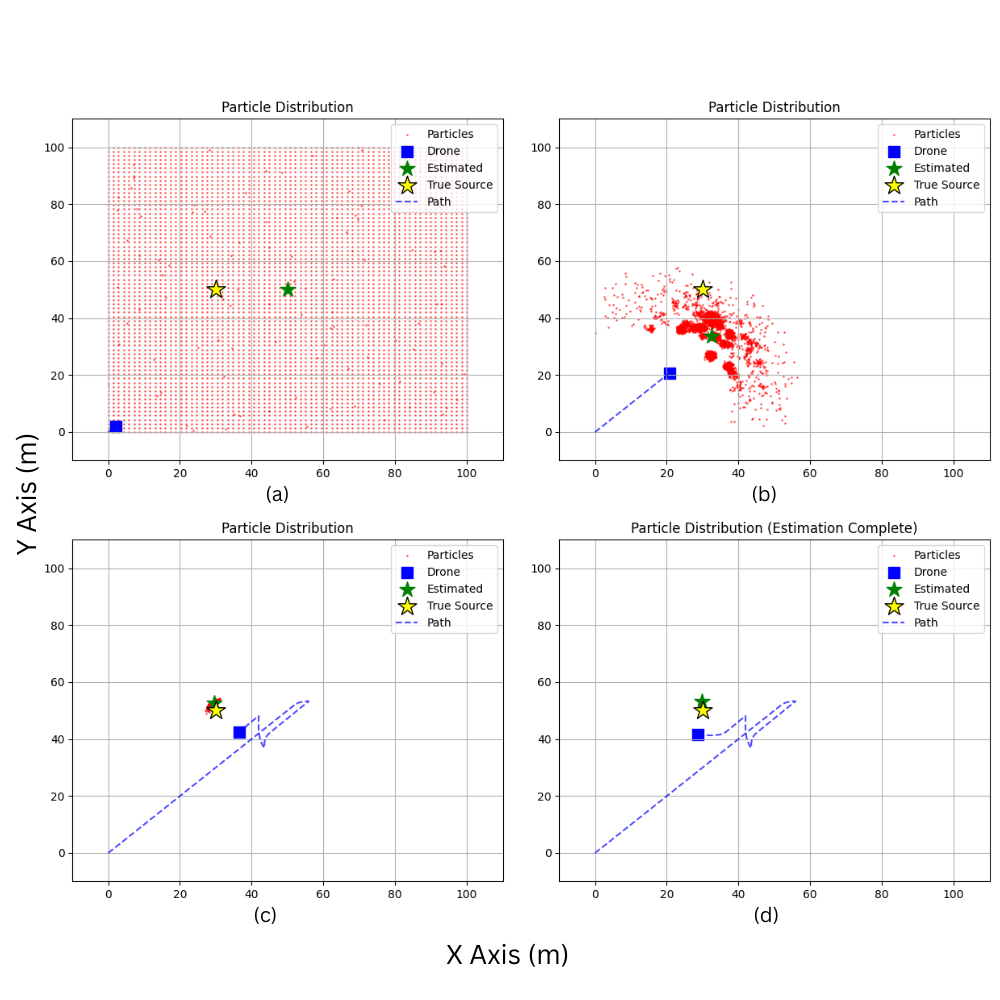
\includegraphics[width=\linewidth]{figures/entropy_algorithm_with_label.png}
        \caption{Information gain-based radiation source localization for source location (30, 50): a. Initial particle distribution across search area, 
        b. Particle resampling on source detection, 
        c. Convergence of particles near true source location, and 
        d. Final source position estimation with completed path}
        \label{fig:entropy_algorithm_with_plot}
    \end{figure}

    Figure~\ref{fig:entropy_algorithm_with_plot} represents the run of the information gain-based radiation source localization algorithm for a source located at (30, 50). The 
    particles are uniformly distributed across the search area initially, and the algorithm converges on the true source location after the source has been detected using ~\ref{eq:prob_detection} starting 
    from figure~\ref{fig:entropy_algorithm_with_plot}.b. The final source location theoretically is the point where the  particles converge as in figure~\ref{fig:entropy_algorithm_with_plot}.d.This 
    run localized the source at a distance of 3 meters from the actual source location.


    \subsubsection{Rollout-based Algorithm}

    \paragraph{Belief update methodology}
    The core of this method is the belief update mechanism that transforms the radiation measurements into a probabilistic representation of the source's potential location. This belief update 
    method employs a three-dimensional grid-based representation of the search area, with each grid cell containing a probability value that represents the likelihood of the source being located.
    For a typical search area of 100 x 100 meters, a grid resolution of 5 meters was selected to balance computational efficiency with localization accuracy. When the grid 
    resolution is too fine, the algorithm may struggle to converge due to the higher number of grid cells, while a coarser resolution may lead to higher prediction error.

    The belief update process begins with computing the likelihood of each measurement given potential source configurations. For a measurement $m_i$ at the drone's position, the likelihood of 
    the measurement given a hypothesized source at position $x_j$ with intensity $I_k$ is modeled as:

    \begin{equation}
        L(m_i | x_j, I_k) = \frac{1}{\sqrt{2\pi\sigma^2}} \exp\left(-\frac{(m_i - \hat{m}(x_j, I_k))^2}{2\sigma^2}\right)
        \label{eq:rollout_likelihood}
    \end{equation}

    Here, $\sigma$ represents the measurement uncertainty, which scales proportionally with the expected measurement intensity: $\sigma = 0.5 \cdot \hat{m}(x_j, I_k)$. This scaling captures the physical reality that measurement noise increases with radiation intensity.

    The expected measurement $\hat{m}(x_j, I_k)$ is computed using the inverse square law for radiation propagation, incorporating the drone's height $h$ for accurate distance calculations:

    \begin{equation}
        \hat{m}(x_j, I_k) = \frac{I_k}{(x - x_j)^2 + (y - y_j)^2 + h^2}
    \end{equation}

    Where $(x,y)$ represents the drone's position, $(x_j,y_j)$ represents a potential source location, and $I_k$ is the hypothesized source intensity. This equation reflects how 
    radiation intensity decreases with the square of the distance from the source, just as light spreads out from a point source.
    
    The system updates its belief state using Bayes' rule, which combines the likelihood of new measurements with prior beliefs:
    \begin{equation}
        P(x_j, I_k|M) = \frac{P(M|x_j, I_k)P(x_j, I_k)}{\sum_{j,k} P(M|x_j, I_k)P(x_j, I_k)}
    \end{equation}
    Where $P(x_j, I_k|M)$ is the posterior probability over position and intensity, $P(M|x_j,I_k)$ is the measurement likelihood, and $P(x_j,I_k)$ is the prior probability.

    The belief confidence, which is crucial for detection and convergence checking, is calculated as the maximum posterior probability across all grid cells and intensities:
    \begin{equation}
        \text{confidence} = \max_{j,k} P(x_j, I_k|M)
    \end{equation}

    The algorithm uses this confidence measure, along with several other important metrics, to make key decisions about source detection and convergence. During the exploration phase, source detection 
    is determined through three key criteria that work together. First, the belief confidence must exceed 0.50, indicating a reasonable level of certainty in the source location. Second, the system 
    must have collected at least five measurements to ensure sufficient data for reliable detection. Third, the algorithm checks for stability in the source position estimate - specifically, the 
    maximum likelihood estimate of the source position must not change by more than 5 meters between consecutive updates. This stability check helps prevent false detections due to temporary 
    measurement anomalies.
   
    The final convergence requirements are noticeably stricter and are intended to guarantee high-confidence radiation source localization. The source location estimate must be extremely certain, 
    as the belief confidence threshold is increased to 0.95. To ensure that the final estimate is supported by a solid dataset, the minimum number of measurements is doubled to ten. The position 
    estimate's stability requirement is raised by the requirement that the maximum likelihood estimate remain within two meters of its previous value. The drone must be within two meters of the 
    estimated source location, according to the algorithm's additional requirement for physical proximity. This proximity criterion is particularly important since it allows the system to acquire
     high-quality, last-minute measurements up close, which is crucial for verifying the source location estimate.

    \paragraph{Rollout Implementation}
    The rollout algorithm in dynamic optimization problems represents a form of approximate dynamic programming that uses a base heuristic through lookahead and policy iteration \cite{bertsekas2013rollout}. 
    A rollout algorithm simulates multiple trajectories that represent possible future states from the current state, uses the base heuristic to evaluate these trajectories, and chooses the 
    action that maximizes the objective. This algorithm was implemented for the localization of radioactive sources by guiding the UAV to utilize a rollout-based path planning strategy to select 
    the next best position to move. This algorithm borrows concepts and observations from previous works by Hoffmann et al. \cite{rolloutHoffmann2019} and Tian et al. \cite{rolloutMultiStepLookaheadTian2008}

    While Hoffmann et al. focused on bearing only RF emitter localization, the approach for radiation source localization needed some adaptations as it had to account for the challenges in localizing 
    radiation sources. Where the original work focussed on optimizing bearing measurements and movement costs, our approach needed to account for radiation characteristics such as
    inverse square law decay, intensity estimation, and radiation attenuations. The intensity estimation is relevant here as the algorithm does not have prior knowledge of the source intensity. 
    Hoffmann et al. use a Q-value $ Q(s, a) $, which is basically the expected cumulative reward of taking action in state $s$ and following an optimal policy thereafter. In their work, 
    The Q-value is estimated by considering the immediate cost, combining movement and measurement time, and the expected future cost, which is again considered the movement and measurement time.
    
    
    To adapt the Q-value computation for radiation-specific physics and simulated radiation measurements, the following modifications were done:

    \begin{equation}
        Q(s_t,a_t) = \sum_{t=0}^{T} \gamma^t V(s_t, m_t)
    \end{equation}
    where $ V(s_t,m_t) $ is the value function combining belief values and simulated radiation measurements:
    \begin{equation}
        V(s_t,m_t) = \frac{\sum_{i,j \in M}b(i,j)}{1 + d(s_t, x_{i,j})} + \frac{1}{1 + 0.2*d\_max}
    \end{equation}

    where $ m_t $ is the simulated measurements at time t, $\gamma = 0.9$ is the discount factor, $b(i,j)$ is the belief at grid cell $(i,j)$, $s_t$ represents the state 
    (drone position and belief) at time $t$, and $a_t$ represents the action (movement) being evaluated, $d(s_t, x_{i,j})$ is the distance from state $s_t$ to grid cell $(i,j)$,
    $d\_max$ is the distance to the maximum belief point, $T$ is the planning horizon and $M$ represents the set of grid cells within the search area boundaries.
    The discount factor $\gamma$ helps balance between immediate and future rewards, ensuring that the cumulative reward does not grow unbounded and thereby making the 
    comparison between trajectories more meaningful. Furthermore, the discount factor helps to retain the focus on early rewards in the trajectory than later, as it may contain crucial 
    information that can guide the estimation. 

    To evaluate these Q-values in practice, the rollout algorithm performs trajectory planning by generating multiple candidate trajectories from the drone's current position. At each decision 
    point,  the algorithm calculates a set of possible movement angles based on the current belief state and drone position, after which the algorithm simulates multiple potential paths with 
    adaptive step sizes. Each simulated path allows the algorithm to compute the corresponding Q-value by evaluating the value function along the trajectory, accounting for both immediate 
    measurement potential and future exploration value. This systematic evaluation of possible trajectories through Q-value computation allows the system to make decisions that balance the 
    immediate need for information with the strategic value of maintaining efficient coverage of the search area.


    The exploitation phase continues until strict convergence criteria are met: the belief confidence must exceed 0.95, the maximum likelihood estimate must remain stable across multiple 
    measurements, and the drone must confirm proximity to the estimated source location through direct measurements. This systematic evaluation of possible trajectories through Q-value 
    computation allows the system to make decisions that balance the immediate need for information with the strategic value of maintaining efficient coverage of the search area.
    \begin{figure}[ht]
        \centering
        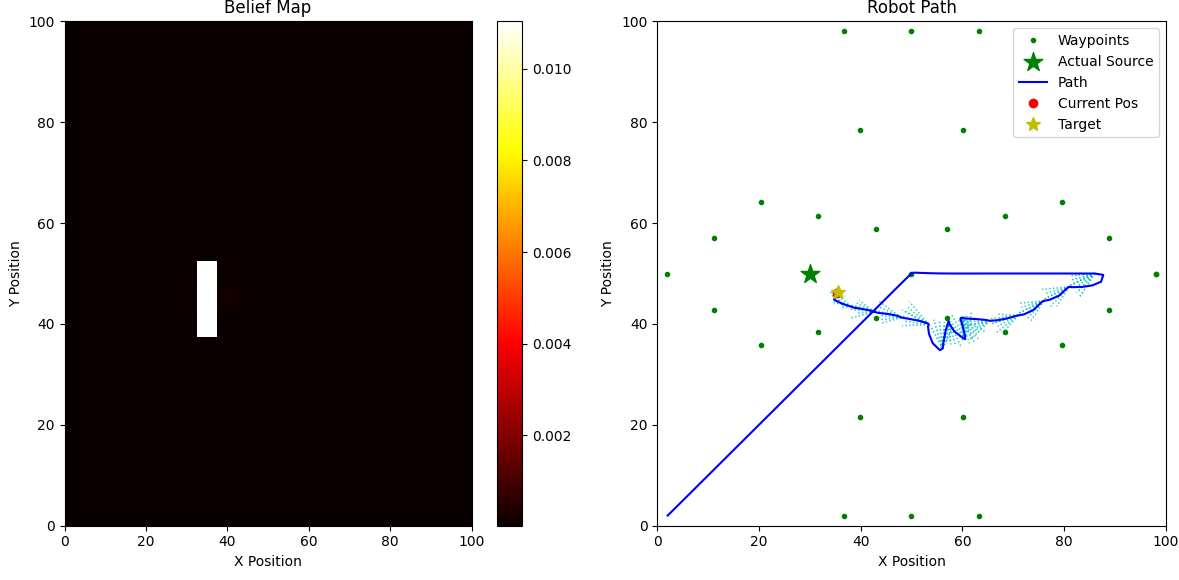
\includegraphics[width=\linewidth]{figures/rollout_algorithm.png}
        \caption{Rollout algorithm-based radiation source localization for source location (30, 50)}
        \label{fig:rollout_algorithm_plot}
    \end{figure}

    Figure~\ref{fig:rollout_algorithm_plot} represents the run of the rollout algorithm-based radiation source localization algorithm for a source located at (30, 50). The blue line represents 
    the path taken by the drone, the blue dotted line represents the trajectory rollouts from the current position and the yellow start at the end of each algorithm-chosen trajectory endpoint
    position. This run localized the source at a distance of 7 meters from the actual source location. 

    \subsubsection{Inverse Square Law Optimization}
    The implemented localization method is based on the inverse square law for radiation intensity and serves as a deterministic baseline for comparing different 
    radiation source search strategies. The algorithm employs a concentric search pattern that scales automatically according to the search area consisting of 
    three concentric circles positioned at 25\%, 50\%, and 75\% of the search area radius. This pattern begins from the center and expands outward, with the number 
    of measurement points per circle scaling proportionally with the map size to maintain consistent coverage across different search areas. The choice of using 
    concentric circles for data collection is based on tests showing that other patterns, such as shamrock, were less effective in terms of coverage and accuracy. 
    This approach balances the need to collect data covering most of the search space with the constraint of avoiding excessive time consumption.

        % The localization process relies on collecting radiation measurements at predefined points along this spiral trajectory. The source position estimation utilizes a weighted optimization 
        % approach incorporating the inverse square law, with higher weights assigned to stronger radiation readings to improve accuracy. To handle uncertainty in source intensity, the algorithm 
        % employs multiple optimization attempts with varying initial intensity estimates (100x, 1000x, and 10000x the maximum measured count rate) to avoid local minima. The uncertainty is further
        % quantified through a confidence circle around the estimated source position, with its radius proportional to the standard deviation of measurements. The uncertainty is further quantified 
        % through a confidence circle around the estimated source position, with its radius proportional to the standard deviation of measurements. The Nelder-Mead optimization method constrained 
        % to the defined search area processes these measurements to determine the most likely source position and intensity within bounded parameters.

    This method localizes the radiation source by beginning with deciding the search pattern and number of measurement points on this pattern scale based on the map size. At each
    measurement point, the radiation sensors collect radiation count and compare it against the expected measurements based on the inverse square law, which dictates that the intensity 
    decreases with the square distance from the source. These measurements are then weighted, assigning higher importance to stronger readings, as they indicate the proximity 
    to the source. The collected data is fed into the Nelder-Mead optimization algorithm, which iteratively adjusts the source position and intensity by minimizing the log-space error
    between the expected and measured radiation counts. To handle uncertainty in source intensity, the algorithm employs multiple optimization attempts with varying initial intensity estimates 
    (100x, 1000x, and 10000x the maximum measured count rate) to avoid local minima. The final estimated source location comes with a confidence circle, where the radius corresponds to the standard deviation of the measurements,
     reflecting the level of uncertainty associated with the estimate.

        
    Many real-world problems involve objective functions that are not differentiable due to noise, discontinuities, and radiation measurements are one of those 
    problems. Gradient-based optimization methods struggle with such functions as they need smooth, differentiable functions to work. The Nelder-Mead algorithm is 
    effective for non-smooth or discontinuous functions because it does not rely on gradients. Instead, it evaluates the function at simplex vertices and adjusts the 
    simplex shape iteratively. This makes it a robust choice for optimization problems where derivative information is unavailable or unreliable. Compared to global optimization methods 
    like evolutionary algorithms, the Nelder-Mead approach offers lower computational costs for problems with fewer variables or limited evaluations, which aligns 
    well with the requirements of engineering optimization. \cite{luersen2004constrained}


    This approach is an effective baseline for comparison due to its deterministic nature, foundation in established physics principles, reproducible 
    behavior, and comprehensive evaluation metrics. The predefined path strategy and inverse square law optimization provide a methodical reference
    point against which more sophisticated, informed search strategies can be evaluated.
    
    \begin{figure}[ht]
        \centering
        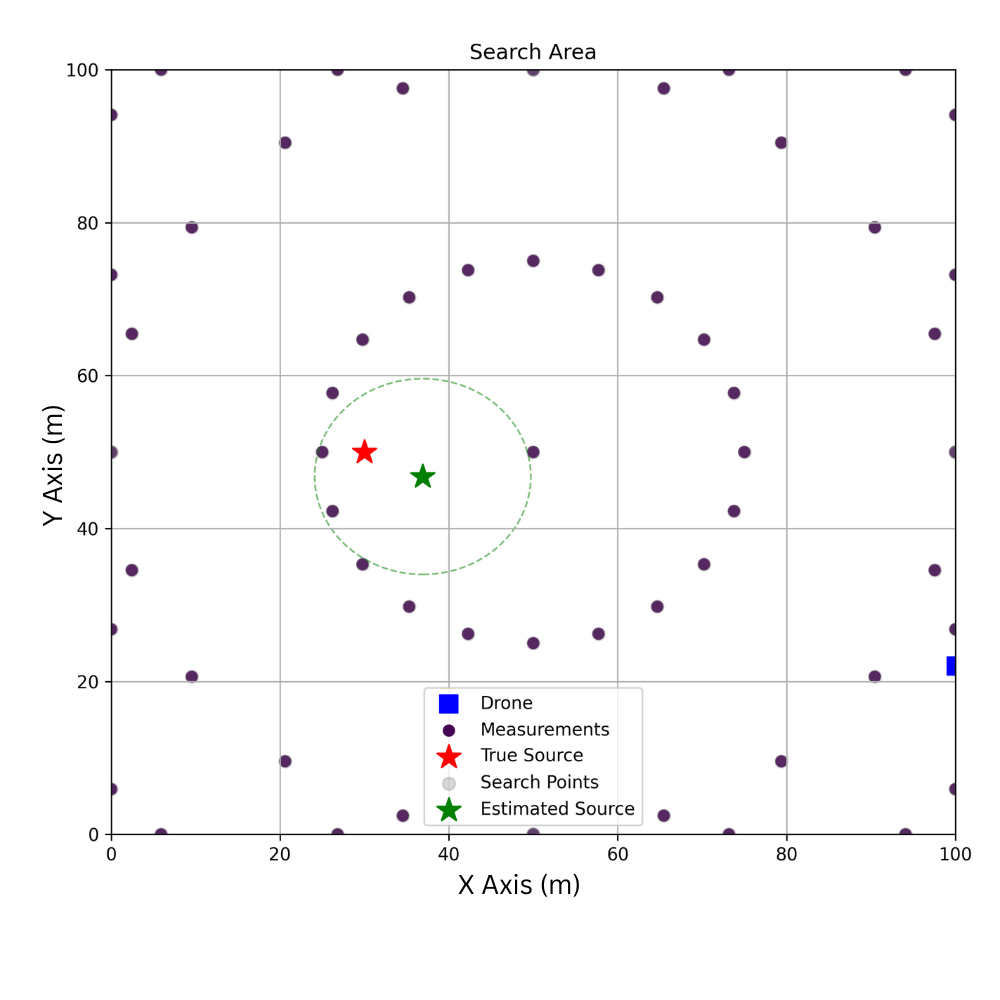
\includegraphics[width=\linewidth]{figures/inverse_square_method_with_label.png}
        \caption{inverse square optimization-based radiation source localization for source location (30, 50)}
        \label{fig:inverse_square_method_plot}
    \end{figure}

    Figure~\ref{fig:inverse_square_method_plot} represents the run of the inverse square law optimization-based radiation source localization algorithm for a source located at (30, 50). the green 
    ellipse represents the confidence circle around the estimated source position(green star). The red star represents the true source position, the black points represent the visited measurement points, and 
    the blue square represents the estimated source position. This run localized the source at a distance of 7.6 meters from the actual source location.

    



\end{document}
